\documentclass[a4paper,10pt]{article}
\usepackage[margin=1in]{geometry}
\usepackage{polski}
\usepackage[utf8x]{inputenc}
\usepackage[unicode]{hyperref}
\usepackage{amssymb}
\usepackage{xifthen}
\usepackage[fleqn]{amsmath}
\usepackage{todonotes}
\usepackage{graphicx}
\usepackage{float}
\usepackage{fullpage}
\usepackage{epstopdf}
\usepackage{multirow}
\usepackage{subfig}
\usepackage[europeanresistors,americaninductors]{circuitikz}
\usetikzlibrary{patterns}
\newcommand{\withtodo}{0}

\def\arraystretch{1.2}

\begin{document}

\begin{table}
  \centering
  \def\arraystretch{1.5}
    \begin{tabular}{|l|l|l|l|} \hline
    Wydział:           & \multicolumn{2}{l|}{Dzień:Poniedziałek 14-17}    &Zespół:  \\
    Fizyki             &    \multicolumn{2}{l|}{Data: 13.03.2017}         &8             \\\hline
    Imiona i nazwiska: &Ocena z przygotowania:  &Ocena ze sprawozdania:   &Ocena końcowa: \\
    Marta Pogorzelska  &                        &                         &                \\
    Paulina Marikin    &                        &                         &\\\hline
    \multicolumn{2}{|l|}{Prowadzący:                 } &\multicolumn{2}{l|}{Podpis:             }  \\\hline
  \end{tabular}
\end{table}


\section{Cel badań}
\paragraph{Zapoznanie się  z założeniami rozkładu Maxwella dla gazu doskonałego oraz sprawdzić poprawność zastosowania jej do opisu zbioru elektronów termicznych.}...

\section{Wstęp teoretyczny}
\paragraph{Rozkład Maxwella zakłada, że cząsteczki powietrza, a dokładniej gazu doskonałego, nie poruszają się z taką samą
prędkością, tylko ich  wartości są różne i zawierają się w pewnym przedziale prędkości $<v, v + dv>$. Według teg
o założenia zamiast mówić o prędkości pojedynczych cząsteczek gazu, mówimy o rozkładzie prędkości tych cząsteczek
. Statystyka Maxwella pokazuje również, że prędkości tych cząsteczek oraz ich rozkład zależą  od temperatury. Wra
z ze wzrostem temperatury rozkład poszerza się i spłaszcza a prędkości cząsteczek zwiększają się.

 Opisany powyżej rozkład można zastosować  do opisu zbioru elektronów termicznych emitowanych przez katodę lampy
elektronowej. Wynika to ze zjawiska termoemisji oraz przybliżenia gazu elektronowego do gazu doskonałego. Podsta
wą do takich założeń, jest między innymi fakt, że koncentracja elektronów, które opuściły metal jest znacząco mni
ejsza niż tych pozostałych w metalu. Pozwala to na zaniedbanie oddziaływań między tymi cząsteczkami.

 Rozkład prędkości elektronów termicznych można wyznaczyć między innymi na podstawie pomiarów prądu anodowego w
funkcji napięcia hamującego, co zostanie wykorzystane w tym doświadczeniu.

 Zależność między prądem anodowym Ia i napięciem Ua można zapisać wzorem:}

\begin{equation}
  I_a(U_a) = I_{a0}\exp{\Big(\frac{-eU_a}{kT}\Big)}
\end{equation}
\paragraph{gdzie $I_{a0}$ – prąd anodowy przy napięciu $U_a = 0$, $k$ – stała Boltzmanna, $T$ – temperatura lampy  próżnio
wej wyrażona w Kelwinach,

 $e$ - ładunek elementarny.}

\section{Metoda przeprowadzenia badań i pomiarów, materiały, aparatura}
{Aparatura pomiarowa}
\begin{itemize}
  \item Woltomierz cyfrowy klasy 0.3
  \item Amperomierz analogowy klasy 1.5
  \item Amperomierz cyfrowy klasy 0.3
\end{itemize}
{Pozostałe elementy}
\begin{itemize}
  \item Kable
  \item Lampa próżniowa
	\item Dzielnik napięcia
\end{itemize}
\paragraph{Najpierw należało połączyć elementy układu według schematu przedstawionego powyżej. Po dokładnym sprawdzeniu podłączenia układu przyrządy zostały włączone. Następnie ustawiony został prąd żarzenia lampy elektronowej wyznaczony przez prowadzącego. Po odczekaniu kilku minut i ustaleniu się wartości prądu żarzenia wykonano pomiary wartości prądu anodowego w zależności od napięć między katodą i anodą. Wykonano dwie serie dla dwóch różnych wartości prądu żarzenia pamiętając, aby wartości pomiarów prądu anodowego nie spadły poniżej $\frac{1}{3}$ początkowej wartości. Po każdej serii, przy zmianie prądu żarzenia, odczekano kilka minut w celu ustabilizowania się jego wartości.}

\begin{figure}[H]
\includegraphics[width=0.5\textwidth]{Schemat.png}
\end{figure}


\section{Wyniki pomiarów}

\begin{tabular}{|l|r|r|r|r|}
\toprule
\hline
{} &\multicolumn{2}{c|}{Seria 1} &\multicolumn{2}{c|}{Seria 2}\\\hline
{} &\multicolumn{2}{c|}{I$_ż$ = 0.448(2)A} &\multicolumn{2}{c|}{I$_ż$ = 0.528(3)A}\\\hline
{} &  U$_a$[mV] &  I$_a$[$\mu$A] &  U$_a$[mV] &  I$_a$[$\mu$A] \\\hline
\midrule
0  &     -0.0(1) &        15 &     -0.7(1) &       150 \\\hline
1  &    -10.2(1) &        14 &    -14.3(1) &       140 \\\hline
2  &    -16.9(2) &        13 &    -30.2(2) &       130 \\\hline
3  &    -24.9(2) &        12 &    -47.2(2) &       120 \\\hline
4  &    -32.9(2) &        11 &    -63.5(3) &       110 \\\hline
5  &    -42.4(2) &        10 &    -79.5(3) &       100 \\\hline
6  &    -51.9(3) &         9 &    -98.3(4) &        90 \\\hline
7  &    -63.7(3) &         8 &   -116.5(4) &        80 \\\hline
8  &    -75.0(3) &         7 &   -136.4(5) &        70 \\\hline
9  &    -89.3(4) &         6 &   -157.8(6) &        60 \\\hline
10 &   -104.6(4) &         5 &   -181.2(6) &        50 \\\hline
\bottomrule
\end{tabular}

\begin{tabular}{|c c|}
  \toprule

  \hline
  $\ln{\frac{I_a}{I_{a0}}}$ &Niepewnosc \\
  \midrule
   0.00  &0.02  \\\hline
  -0.069 &0.022 \\\hline
  -0.143 &0.023 \\\hline
  -0.223 &0.024 \\\hline
  -0.31  &0.03  \\\hline
  -0.41  &0.03  \\\hline
  -0.51  &0.03\\\hline
  -0.63  &0.03\\\hline
  -0.76  &0.04\\\hline
  -0.92  &0.04\\\hline
  -1.09  &0.05\\\hline
  \bottomrule
\end{tabular}
\\Aby sprawdzić poprawność postawionej tezy wykreślono wykresy zależności(1) dla obu serii i dopasowano do nich
proste jednoparametrowe ($y=ax$) przy użyciu funkcji \emph{curvefit} biblioteki \emph{scipy.optimize} w Pythonie
\begin{figure}[H]
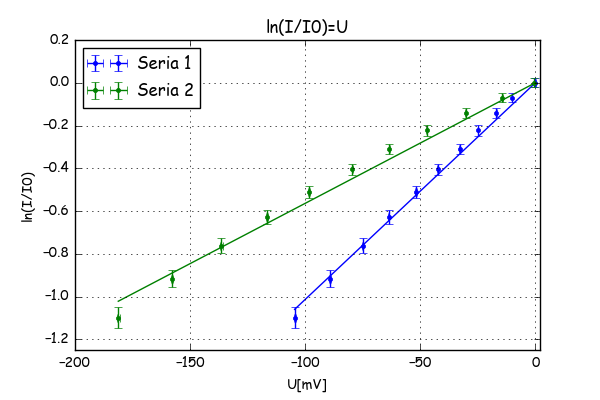
\includegraphics[width=0.9\textwidth]{zarzenie.png}
\end{figure}

\begin{itemize}
  \item Seria 1: $a = 0.01013(13)$
  \item Seria 2: $a = 0.00563(12)$
\end{itemize}

Zgodnie z postawioną teorią współczynnik proporcjonalnoci $a = \frac{-e}{kT}$, znając go można więc wyznaczyć t
emperaturę lampy próżniowej $T = \frac{-e}{ka}$.
\begin{itemize}
  \item $T_1 = 1145(15)$K
  \item $T_2 = 2057(43)$K
\end{itemize}

\begin{figure}[H]
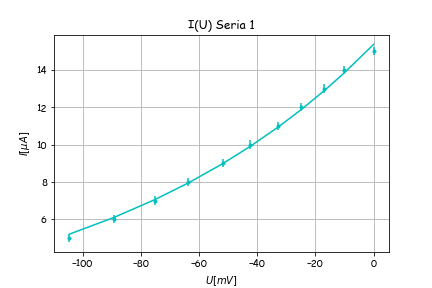
\includegraphics[width=0.5\textwidth]{zarzenieU1.png}
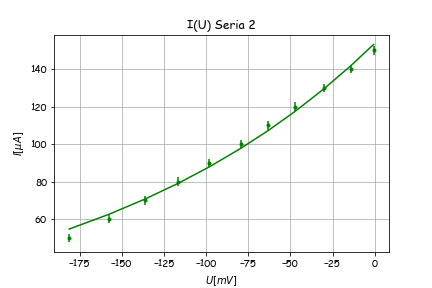
\includegraphics[width=0.5\textwidth]{zarzenieU2.png}
\caption{Wykresy zależności $I(U)$}
\end{figure}

\begin{figure}[H]
 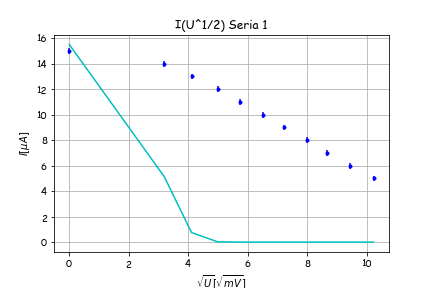
\includegraphics[width=0.5\textwidth]{zarzenieU12.png}
 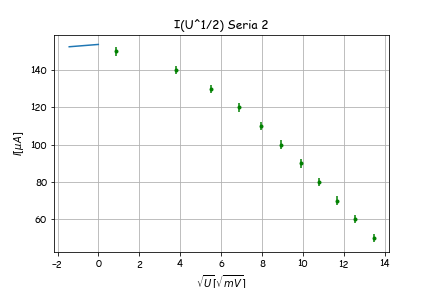
\includegraphics[width=0.5\textwidth]{zarzenieU22.png}
 \caption{Wykresy zależności $I(U^{\frac{1}{2}})$}
 \end{figure}
\section{Analiza niepewności}
Niepewność wyznaczenia prądu dla obu serii wynosiła odpowiednio $0.25\mu$A i $2.25\mu$A, wyliczona jako iloczyn klasy amperomierza i zakresu pomiarowego.
Za niepewność napięcia wzięto iloczyn danego pomiaru i klasy woltomierza + 1dgt.

Niepewność logarytmów i temperatur została wyznaczona metodą różniczki zupełnej. Niepewność współczynnika propo
rcjonalności jest pierwiastkiem kwadratowym z jedynego składnika macierzy kowariancji zwracanego przez funkcję \e
mph{curvefit}. Wszystkie niepewności są relatywnie małe i zdecydowanie wystarczające dla potrzeb danego doświadcz
enia, nie ma więc powodów do ich poprawy.
 \section{Wnioski}
 Na podstawie wykonanych pomiarów oraz przeanalizowania danych doświadczalnych i wykreślonych na ich podstawie w
ykresów można potwierdzić wstępne założenia o poprawności zastosowania rozkładu Maxwella dla elektronów termiczny
ch. Wykres zależności wartości logarytmu naturalnego unormowanego prądu anodowego $\frac{I_a}{I_{a0}}$ od napięci
a $U_a$ przedstawia zależność liniową co skłania ku potwierdzeniu tezy.
 \end{document}
